\documentclass[12pt]{article}
\usepackage{amsmath}
%\usepackage{mathtext}
\usepackage[french]{babel}
\usepackage{amsthm}
\usepackage{arydshln}
\usepackage{nccrules}

\usepackage{amsfonts}
\usepackage{amssymb}
\usepackage{latexsym}
\usepackage{eufrak}
\usepackage{tocloft}
\usepackage[center]{titlesec}
\usepackage[utf8]{inputenc}

%Для рисунков
\usepackage{graphicx}
\usepackage{graphics}
\usepackage{float}
\usepackage{caption}
\usepackage{topcapt}

%\usepackage{citesort}

%%%%%%%%%%%%%%%%%% DEFINE NEW COUNTERS %%%%%%%%%%%%%%%%%%%%%%%%%%%%%
\newcounter{isElectronicVersion} % Must be set as 1 if the electronic version with animations is to be created, otherwise the printed version will be created

%%%%%%%%%%%%%%%%%% SET NEW COUNTERS %%%%%%%%%%%%%%%%%%%%%%%%%%%%%
\setcounter{isElectronicVersion}{0} % 1 - electronic, 0 - printed

%%%%%%%%%%%%%%%%%% MATH OPERATORS %%%%%%%%%%%%%%%%%%%%%%%%%%%%%
\DeclareMathOperator\dv{div} % divegence
\DeclareMathOperator\id{I}   % identity matrix
\DeclareMathOperator\tr{tr}   % trace operator
\DeclareMathOperator\sgn{sgn}   % signum operator
%%%%%%%%%%%%%%%%%% BOLD SYMBOLS %%%%%%%%%%%%%%%%%%%%%%%%%%%%%
\newcommand{\bu}{\mathbf{u}}  % bold u
\newcommand{\bV}{\mathbf{V}}  % bold V
\newcommand{\bU}{\mathbf{U}}  % bold U
\newcommand{\bt}{\mathbf{t}}  % bold t
\newcommand{\bq}{\mathbf{q}}  % bold q
\newcommand{\bx}{\mathbf{x}}  % bold x
\newcommand{\be}{\mathbf{e}}  % bold e
\newcommand{\bbs}{\mathbf{s}}  % bold n
\newcommand{\bn}{\mathbf{n}}  % bold n
\newcommand{\bp}{\mathbf{p}}  % bold p
\newcommand{\bc}{\mathbf{c}}  % bold c
\newcommand{\bs}{\mathbf{s}}  % bold s
\newcommand{\cB}{{\cal B}} % calligraphic B
\newcommand{\mx}{\mathrm{max}}  % roman max
\newcommand{\mn}{\mathrm{min}}  % roman min
\newcommand\norm[1]{\left\lVert#1\right\rVert}
\newcommand{\bcu}{\mathbf{U}} % bold U
\newcommand{\bct}{\mathbf{T}} % bold T
\newcommand{\bpsi}{\bm{\psi}} % bold psi
\newcommand{\bsigma}{\bm{\sigma}} % bold sigma
\newcommand{\btau}{\bm{\tau}} % bold tau
%%%%%%%%%%%%%%%%%% CALLIGRAPHIC SYMBOLS %%%%%%%%%%%%%%%%%%%%%%%%%%%%%
\newcommand{\epss}{{\cal E}}
\newcommand{\cL}{{\cal L}}
\newcommand{\cT}{{\cal T}}
\newcommand{\cQ}{{\cal Q}}

%%%%%%%%%%%%%%%%%% DIFFERENTIAL OPERATORS %%%%%%%%%%%%%%%%%%%%%%%%%%%%%
\newcommand{\pd}[2]{ % partial first derivative
	\dfrac{\partial #1}{\partial #2}
} 
\newcommand{\opd}[2]{ % ordinary first derivative
	\dfrac{\mathrm{d} #1}{\mathrm{d} #2}
}
\newcommand{\pddB}[2]{ % partial first derivative with function bordered by braces
	\dfrac{\partial }{\partial #2}\Bigl(#1\Bigr)
} 
\newcommand{\pdd}[3]{ % partial second derivative
	\dfrac{\partial^2 #1}{\partial #2 \partial #3}
} 
%%%%%%%%%%%%%%%%%% NORM OPERATORS %%%%%%%%%%%%%%%%%%%%%%%%%%%%%
\newcommand{\normInf}[1]{|#1|_\infty} % infinity-norm

\newtheorem{dfn}{Definition}

\graphicspath{{img/}}

%Точечки в Содержании
\renewcommand{\cftsecleader}{\cftdotfill{\cftdotsep}}

%Центрирование Содержания
\renewcommand\cfttoctitlefont{\hfill\Large\bfseries}
\renewcommand\cftaftertoctitle{\hfill\mbox{}}

%Точка после Разделов в Содержании
\let \savenumberline \numberline
\def \numberline#1{\savenumberline{#1.}}

\begin{document}	
	\tableofcontents
	%\title{Influence of inhomogeneity of reservoir to the development of a hydraulic fracture in poroelastic medium}
	\title{Sofya Sizova, Anastasiya Dulepova}
	\maketitle
	\section{Énoncé du problème}
	On s'intéresse au problème 
	\begin{eqnarray}
	\label{Initial_problem}
	& &\text{Trouver } u \in C^2(0, T; L^2(\Omega)) \text{ telle que}\\[2mm]
	& &\begin{cases}
	\dfrac{\partial^2u}{\partial t^2} - \text{div} (\sigma\nabla u) = f \quad  \text{dans } \Omega \times [0, T_\text{max}]\\
	u|_{t = 0} = u_0 \quad \text{dans } \Omega \\
	\pd{u}{t}|_{t = 0} = u_1 \quad \text{dans } \Omega \\
	\sigma \pd{u}{n} = 0 \quad \text{sur } \partial\Omega \times [0, T_\text{max}]
	\end{cases}
	\end{eqnarray}
En multipliant l'équation \eqref{Initial_problem} par la fonction test $v \in H^1(\Omega)$ et un intégrant sur la domaine de $\Omega$, on obtiens la formulation variationnelle en utilisant les formules de Green. Il faut noter que si la solution forte $u$ de \eqref{Initial_problem} vérifie $u \in C^2(0, T; L^2(\Omega))$, on peut relaxer la régularité de solution en temps et utiliser le fait que
\begin{equation}
\int_\Omega{\dfrac{\partial^2u}{\partial t^2}(x,t) v(x)d\Omega} = \frac{d^2}{dt^2} \int_\Omega{u(x,t) v(x)},
\end{equation}
car la partie droite est bien définie au sens de distribution en raison de régularité suffisante. Donc, on suppose maintenant que $u \in C^1(0, T; L^2(\Omega))$ simplement. Il faut que la fonction $u$ soit $C^1$ minimum, car les conditions initiales doivent pouvoir être définies ponctuellement.  Alors, la formulation variationnelle est suivante
\begin{eqnarray}
\nonumber
& &\text{Trouver u} \in C^1(0, T; L^2(\Omega)) \cap C^0(0, T; H^1(\Omega)) \text { tel que}\\
\label{variationnelle}
& &\begin{cases}
\dfrac{d^2}{dt^2} \int_\Omega {u v d\Omega} + \int_\Omega{\sigma \nabla u \nabla v d\Omega} = \int_\Omega{f v d\Omega} \quad \forall v \in H^1(\Omega) \text{ p.p } t \in (0,T),\\
u(x, 0) = u_0, \quad \pd{u}{t}(x,0) = u_1 \quad \text{dans } \Omega \\
\sigma \pd{u}{n} = 0, \text{sur } \partial\Omega \times [0, T_\text{max}]
\end{cases}
\end{eqnarray}


Pour obtenir l'identité d'énergie on multiple la première équation de   \eqref{Initial_problem} par $\pd{u}{t}$ et intègre sur $\Omega$. Donc
\begin{equation}
\label{energie1}
	\int_\Omega{\dfrac{\partial^2u}{\partial t^2} \pd{u}{t} d\Omega} - \int_\Omega{\text{div}(\sigma \nabla u)\pd{u}{t} d\Omega} = \int_\Omega{f \pd{u}{t} d\Omega}.
\end{equation}
On peut modifier le première terme de \eqref{energie1} comment
\begin{equation}
	\int_\Omega{\dfrac{\partial^2u}{\partial t^2} \pd{u}{t} d\Omega}= \frac{1}{2}\int_\Omega{\frac{d}{dt}(\pd{u}{t})^2d\Omega} = \frac{1}{2}\frac{d}{dt}\int_\Omega{(\pd{u}{t})^2d\Omega} = \frac{1}{2}\frac{d}{dt}\|\pd{u}{t}\|^2_{L^2(\Omega)}.
\end{equation}
La deuxième égalité est admissible car la régularité de $u$ est suffisante selon les hypothèses ci-dessous.
Le second terme de \eqref{energie1} est égal à $\int_\Omega{\sigma \nabla u \nabla(\pd{u}{t}) d\Omega}$ après l'équation \eqref{variationnelle} avec $v = \pd{u}{t}$. Donc, on peut s'amener 
\begin{multline}
	\int_\Omega{\sigma \nabla u \nabla(\pd{u}{t}) d\Omega} = \int_\Omega{\sigma \nabla u\pd{\nabla u}{t} d\Omega} = \int_{\Omega}{\frac{d}{dt}\frac{1}{2}(\sqrt{\sigma}\nabla u)^2} =\\ \frac{1}{2}\frac{d}{dt}\int_{\Omega}{(\sqrt{\sigma}\nabla u)^2} \text{ par hypothèses de régularité }
	= \frac{1}{2}\frac{d}{dt}\|\sqrt{\sigma}\nabla u\|^2_{L^2(\Omega)}.
\end{multline}
Donc, l'énergie est définie par $E(t) = \dfrac{1}{2}\|\pd{u}{t}\|^2_{L^2(\Omega)} + \dfrac{1}{2}\|\sqrt{\sigma}\nabla u\|^2_{L^2(\Omega)}$, et on a l'identité
\begin{eqnarray}
& &\dfrac{d E(t)}{dt} = (f(t),\pd{u}{t})_{L^2(\Omega)}, \quad\text{ou} \\[2mm]
& &E(t) = \int_\Omega{f \pd{u}{t}d\Omega} + E_0.
\end{eqnarray}
Si $f = 0$, alors $E = E_0 = \frac{1}{2}\|u_1\|^2 + \frac{1}{2}\|\sqrt{\sigma}\nabla u_0\|^2$, l'énergie se conserve dans le système ferme.
\section{Discrétisation}
Maintenant on discrétise cette formulation variationnelle par les éléments finis de Lagrange $P^1$ en espace et différences finies centrées d’ordre 2 en temps. On va tout d'abord discrétiser l'espace en utilisant le méthode de Galerkin. Soit $V_h$ est de dimension fini et $V_h \subset H^1(\Omega)$, qui vérifie la propriété d'approximation,c'est à dire quand $h$ tend vers 0, $\inf_{v_h\in V_h}\|v - v_h\|$ tend vers zéro $\forall v \in H^1(\Omega)$. Alors, la formulation variationnelle semi-discrète est
\begin{eqnarray}
\nonumber
& &\text{Trouver } u_h \in C^1(0, T; V_h) \text{ tel que}\\[2mm]
\label{semi-discrete}
& &\begin{cases}
\dfrac{d^2}{dt^2} \int_\Omega {u_h v_h d\Omega} + \int_\Omega{\sigma \nabla u_h \nabla v_h d\Omega} = \int_\Omega{f v_h d\Omega} \quad \forall v_h \in V_h \text{ p.p } t \in (0,T),\\
u_h(0) = u_{h,0}, \quad \frac{d u_h}{dt}(0) = u_{h,1} \quad \text{dans } \Omega \\
\sigma \pd{u}{n} = 0, \text{sur } \partial\Omega \times [0, T_\text{max}]
\end{cases}
\end{eqnarray}
On introduit la base de $V_h$ $(\omega_i)_{i = 1..N}$, où $N = \dim{V_h}$. Donc, on peut écrire $u_h$
\begin{equation}
u_h(t) = \sum_{i = 1..N}{u_h(M_i, t)\omega_i} = \sum_{i = 1..N}{U_i(t)\omega_i}.
\end{equation} 
Alors, on peut réécrire la formulation \eqref{semi-discrete} dans une forme matricielle
\begin{eqnarray}
\label{matr_semi_discrete}
	& &\mathbb{M}\frac{d^2U}{dt^2}(t) + \mathbb{K}^\sigma U(t) = F(t)\\
	& &U(0) = U_0, \quad \frac{dU}{dt}(0) = U_1,
\end{eqnarray}
où $\mathbb{M}_{ij} = \int_\Omega{\omega_i \omega_j d\Omega}$, $\mathbb{K}_{ij}:\sigma = \int_\Omega{\sigma\nabla\omega_i \nabla\omega_j d\Omega}$ sont les matrices symétriques, (car $(\mathbb{M}V,V) = \|v_h\|^2 > 0$, et $(\mathbb{K}V,V) = \|\sigma\nabla v_h\|^2 > 0$) et définies positives (car $\omega_i \in H^1_0 \quad \forall i \text{ et dans cette espace on a l'inégalité de Poincaré}$), $F_j = \int_{\Omega}{f\omega_i d\Omega}$.


Pour la discrétisation en temps on considéré $U_i^k = U_i(t_k)$, donc\\ $u_h^k = \sum_{i = 1..N}U_i^k\omega_i$. On va discrétiser la seconde dérivative dans \eqref{semi-discrete} par le schéma d'ordre 2, le schéma saute-mouton. Donc, l'équation \eqref{matr_semi_discrete} discrétise en temps est
\begin{equation}
\mathbb{M}\dfrac{U^{k+1} - 2U^k + U^{k - 1}}{\Delta t^2} + \mathbb{K}^\sigma U^k = F^k.
\end{equation}
Ici $\Delta t $ = $\frac{T}{M}$, $M$ es le nombre de couches dans le temps.
Il faut définir les conditions initiales dans ce cas. En $t = 0$ on a $u_h(0) = u_h^0 \approx u_{h,0}$. Pour le prochain pas du temps $t_1 = \Delta t$ on utilise la formule de Taylor d’ordre 2
\begin{equation}
u(\Delta t) = u_0 + \Delta t u_1 + \frac{\Delta t^2}{2}\frac{\partial^2u}{\partial t^2}(0) + O(\Delta t^3)
\end{equation}
Pour notre équation initiale \eqref{Initial_problem} cela conduit à 
\begin{multline}
\label{Teylor}
	(u_h(\Delta t), v_h)_{L^2} = (u_h^1, v_h)_L^2 \approx (u_{h,0}, v_h) + \Delta t(\pd{u_h}{t}(0),v_h)_{L^2} +\\ \frac{1}{2}(\Delta t)^2(\frac{\partial^2 u_h}{\partial t^2}(0), v_h)_{L^2}.
\end{multline}
On sait que $(\frac{\partial^2 u_h}{\partial t^2}|_{t = 0}, v_h)_{L^2}  + (\sigma \nabla u^0,\nabla v_h) = (f^0,v_h)_L^2$, donc \\
$(\frac{\partial^2 u_h}{\partial t^2}|_{t = 0}, v_h)_{L^2} = F^0 - \sigma\mathbb{K} U_0$ dans le milieu homogène, où $\sigma = c^2$, comme dans notre cas.
À partir de Taylor on déduit la condition initiale
\begin{equation}
	\mathbb{M}U^1 = \mathbb{M}U_0 + \Delta t\mathbb{M}U_1 - \frac{\Delta t^2}{2}c^2\mathbb{K}U_0 +  \frac{\Delta t^2}{2}F^0.
\end{equation}
L'indice supérieur signifie un pas dans le temps, et inférieur signifie le pas dans espace. Finalement, le schéma totalement discrétise est \eqref{total-discr}.
\begin{eqnarray}
\label{total-discr}
\begin{cases}
\mathbb{M}\dfrac{U^{k+1} - 2U^k + U^{k - 1}}{\Delta t^2} +\sigma \mathbb{K} U^k = F^k,\\
U^0 = U_0,\\
\mathbb{M}U^1 = \mathbb{M}U_0 + \Delta t\mathbb{M}U_1 - \frac{\Delta t^2}{2}c^2\mathbb{K}U_0 +  \frac{\Delta t^2}{2}F^0.
\end{cases}
\end{eqnarray}
On peut accélérer ce schéma en augmentant le pas d'un temps $\Delta t$ ou la taille de discrétisation en espace $h$. Mais il est important de se rappeler que les valeurs arbitraires de $h$ et $\Delta t$ peuvent entraîner une instabilité de schéma. Il faut que ces valeurs satisfassent l'inégalité de stabilité (la condition de Courant–Friedrichs–Levy), qui sera donné ci-dessous.
\section{L'identité d'énergie discrète}
On définit une énergie discrète du schéma $\mathcal{E}$ , qui représente l'approximation de l'énergie continue $E(t)$.
\begin{equation}
	\mathcal{E}^{k + 1/2} = \frac{1}{2}\norm{\frac{U^{k+1} - U^k}{\Delta t}}_\mathbb{M}^2 + \frac{1}{2}(c^2\mathbb{K}U^k, U^{k+1}).
\end{equation}
Ici $\norm{U}_\mathbb{M}^2 = (\mathbb{M}U,U)$. Pour obtenir l'inégalité d'énergie discrète on multiple la première équation de \eqref{total-discr} par $\frac{U^{k+1} - U^{k - 1}}{2\Delta t}$. En regroupant les termes, nous obtenons
\begin{multline}
	\frac{1}{2}\mathbb{M}\frac{(U^{k+1} - U^k)^2 - (U^k - U^{k-1})^2}{\Delta t^2} + \frac{1}{2}(c^2\mathbb{K}U^k, U^{k+1}) - \frac{1}{2}(c^2\mathbb{K}U^{k}, U^{k-1}) \\= \Delta t(F^k, \frac{U^{k+1} - U^{k - 1}}{2\Delta t}).
\end{multline}
En absence de source on obtiens que l'énergie discrète se conserve.
\begin{equation}
\label{energie-discrete}
	\mathcal{E}^{k +1/2} = \mathcal{E}^{k - 1/2} \quad \forall k \geq 1.
\end{equation}
Pour déduire la condition de stabilité à partir d'égalité \eqref{energie-discrete}, il faut s'assurer que $(c^2\mathbb{K}U^k, U^{k+1})$ soit définie positive. Cela conduit à la formulation d'une condition de stabilité nécessaire de type CFL \eqref{CFL1}.
\begin{equation}
\label{CFL1}
\gamma_{\text{cfl}} = \frac{c^2 \Delta t^2}{4}\sup_{V \neq 0} \frac{(\mathbb{K}V, V)}{(\mathbb{M}V, V)} \leq 1.
\end{equation}
On peut utilisé le théorie connu pour exprimer cette condition dans une autre forme.
\begin{eqnarray}
	& &\gamma_{\text{cfl}} = \frac{c^2 \Delta t^2}{4} \sup_i|\lambda_i|, \text{où}\\
	\nonumber
	& &\lambda_i \text{ sont les solution de probleme aux valeurs propres}\\
	\label{propres}
	& &\begin{cases}
	-\text{div}(\sigma\nabla u ) = \lambda u,\\
	\sigma \pd{u}{n} = 0 \quad \text{sur } \partial\Omega
	\end{cases} \\
		\nonumber
	& &\text{ qui est equivalente de la formulation } c^2\mathbb{K}U = \lambda_h \mathbb{M}U.
\end{eqnarray}
Alors, le schéma est stable, si le pas en temps 
\begin{equation}
\label{CFL}
\Delta t \leq \frac{2}{c \sqrt{\sup |\lambda_i|}}.
\end{equation}
Pour donner l'expression plus précise il faut calculer le spectre du problème \eqref{propres}.
\section{Condensation de masse}
L'inconvénient de la formulation \eqref{total-discr} est que le schéma n'est pas explicite et on doit chaque fois inverser la matrice $\mathbb{M}$. On veut approcher la matrice de masse $\mathbb{M}$ par une matrice diagonale en utilisant les formules de quadratures suivante
\begin{equation}
	\int_{\mathcal{T}}{g(x) dT} \approx \frac{|\mathcal{T}|}{3}\sum_{i = 1}^3{g(S_i)},
\end{equation}
où $\mathcal{T}$ est une triangle dans le maillage avec l'aire égal à $|\mathcal{T}|$ et les sommets $S_i, i = 1,2,3$.
Dans le cas du maillage uniforme, $\mathbb{M}^{cond} = h^2I$, $I$ est la matrice unitaire.
Les expressions pour la matrice de rigidité et la matrice de masse sans condensation sont présenté ci-dessous.
\section{Le pas de temps autorise par la condition de CFL}
En résolvant le problème \eqref{propres} numériquement pour le maillage comme dans fig. \ref{fig:maillage1} on a trouvé les plus grandes valeurs propre $\lambda^{sup}_h$ pour $h = 0.02j, j = 1..10$. Donc, par \eqref{CFL} on obtiens l'estimations pour $\Delta t$, qui sont présentés dans le tableaux dessous.
	\begin{figure}
	\centering
	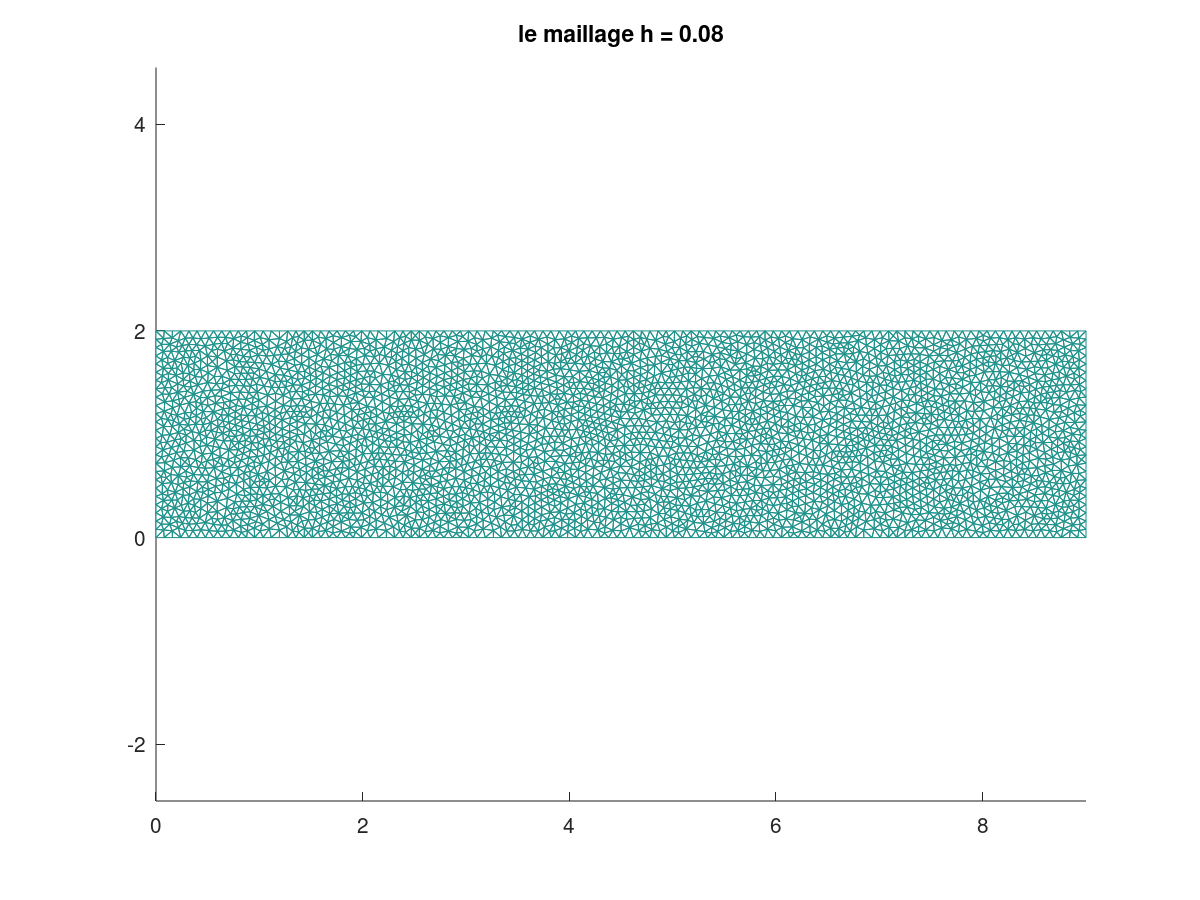
\includegraphics[height=0.4\linewidth]{images/maillage1}
	\caption{La discrétisation de domaine  avec $h = 0.8$.}
	\label{fig:maillage1}
\end{figure}
\begin{table}[H]
	\caption{\label{tab:canonsummary} Le pas de temps maximum autorisé par la condition CFL pour la matrice exacte (gauche) et la matrice condensée (droite) }
	\begin{center}
		\begin{tabular}{|c|c|c|}
			\hline
			$h$ & $\Delta t_{ex}$ & $\Delta t_{cond}$ \\
			\hline
			0.02 & $-$ &  $-$ \\
			0.04 &  $ 0.005$ &  $-$ \\
			0.06 & 0.009 & 12~bit\\
			0.08 & 0.012 &12~bit\\
			0.1  & 0.015 &12~bit\\
			0.12 & 0.018 &12~bit\\
			0.14 & 0.021 &12~bit\\
			0.16 & 0.024 &12~bit\\
			0.18 & 0.028 &12~bit\\
			0.2  & 0.028 &~bit\\
			\hline
		\end{tabular}
	\end{center}
\end{table} 
\section{La partie droite (5.7)}
La partie droite dans \eqref{total-discr} est calculer à l'aide d'une méthode d'interpolation.
\begin{equation}
	F^k = M\tilde{F}^k =\sum_{j = 1..3} Mf(t_k, S_j)
\end{equation}
\end{document}